% The sequence slide 29 sits in: prices -> quantities, quantities by flows,
% then quantities -> prices. Compiled to seq29.png; see slides/img/README.
\documentclass[border=5pt]{standalone}
\usepackage[scaled]{helvet}
\renewcommand\familydefault{\sfdefault}
\usepackage{amsmath}
\usepackage[dvipsnames]{xcolor}
\usepackage{tikz}
\usetikzlibrary{arrows.meta, positioning, calc}
\definecolor{blueA}{HTML}{2A78D6}
\definecolor{orangeA}{HTML}{EB6834}
\definecolor{greenA}{HTML}{1BAF7A}
\definecolor{ink}{HTML}{101519}
\definecolor{ink2}{HTML}{5B6873}
\begin{document}
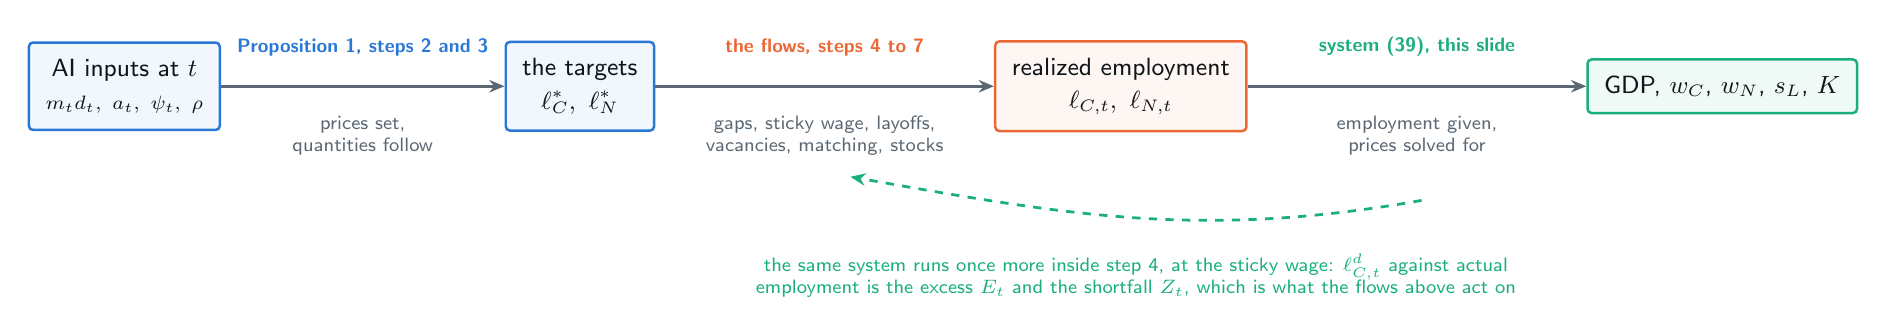
\begin{tikzpicture}[
  font=\small, text=ink,
  bx/.style  ={draw, line width=0.9pt, align=center, inner sep=6pt, rounded corners=1.5pt},
  bl/.style  ={bx, draw=blueA,   fill=blueA!6},
  og/.style  ={bx, draw=orangeA, fill=orangeA!6},
  gr/.style  ={bx, draw=greenA,  fill=greenA!7},
  arr/.style ={-{Stealth[length=5.5pt,width=4.5pt]}, line width=1pt, draw=ink2},
  under/.style={font=\scriptsize, text=ink2, align=center, midway, below=7pt},
  over/.style ={font=\scriptsize\bfseries, align=center, midway, above=7pt},
  note/.style ={font=\scriptsize, align=center, anchor=north}
]
\node[bl] (inp) {AI inputs at $t$\\[1pt] {\scriptsize $m_t d_t,\ a_t,\ \psi_t,\ \rho$}};
\node[bl, right=3.6cm of inp]  (tgt)  {the targets\\[1pt] $\ell^{*}_{C},\ \ell^{*}_{N}$};
\node[og, right=4.3cm of tgt]  (real) {realized employment\\[1pt] $\ell_{C,t},\ \ell_{N,t}$};
\node[gr, right=4.3cm of real] (out)  {GDP, $w_C$, $w_N$, $s_L$, $K$};

\draw[arr] (inp) -- (tgt)
  node[over, text=blueA]{Proposition 1, steps 2 and 3}
  node[under]{prices set,\\quantities follow};
\draw[arr] (tgt) -- (real)
  node[over, text=orangeA]{the flows, steps 4 to 7}
  node[under]{gaps, sticky wage, layoffs,\\vacancies, matching, stocks};
\draw[arr] (real) -- (out)
  node[over, text=greenA]{system (39), this slide}
  node[under]{employment given,\\prices solved for};

% the same system, used once more inside step 4
\coordinate (g) at ($(real)!0.5!(out)$);
\coordinate (f) at ($(tgt)!0.5!(real)$);
\draw[arr, dashed, draw=greenA] ($(g)+(0,-1.45)$) to[out=190, in=-10] ($(f)+(0,-1.15)$);
\node[note, text=greenA] at ($(g)!0.5!(f)+(0,-2.0)$)
  {the same system runs once more inside step 4, at the sticky wage: $\ell^{d}_{C,t}$ against actual\\
   employment is the excess $E_t$ and the shortfall $Z_t$, which is what the flows above act on};
\end{tikzpicture}
\end{document}
